\documentclass[11pt]{article}

% parameters are fairly self-explanatory here, thankfully
\usepackage[width=7in,height=9.5in,top=0.75in,centering]{geometry}

% for math-ing
\usepackage{amsmath}
\usepackage{amssymb}
\usepackage{comment}

%%%%%% tables %%%%%%%%
\usepackage{tabularx}
\usepackage{array}
\renewcommand{\arraystretch}{1.5}
\setlength{\tabcolsep}{8pt}

%%%%%% plotting %%%%%%

\usepackage[dvipsnames]{xcolor}
\usepackage{tikz}
\usepackage{pgfplots}

\pgfplotsset{every axis/.append style={
                    axis x line=middle,    % put the x axis in the middle
                    axis y line=middle,    % put the y axis in the middle
                    axis line style={<->,color=black}, % arrows on the axis
                    xlabel={$x$},          % default put x on x-axis
                    ylabel={$y$},          % default put y on y-axis
            }}
            
 \pgfplotsset{compat=1.14} % sometimes, everything falls apart without this
 
 %\usepgfplotslibrary{fillbetween} %for shading between curves

%%%%%% commands %%%%%%

\def\todo{\textcolor{red}{TODO}}

% exam heading; course name is first argument, exam information is second argument
\newcommand{\Heading}[2]{
    \fbox{
        {\Large\textbf{#1}}
        }
    \hfill
    \fbox{
        \begin{minipage}{0.2\textwidth}
            \begin{center}
            \textbf{#2}
            \end{center}
        \end{minipage}
    }
    \par\vspace{0.1in}}

% for being lazy while beautifying integrals
\newcommand{\dint}{\displaystyle\int}

% for being lazy while beautifying limits
\newcommand{\dlim}{\displaystyle\lim}

%%%%%% stuff %%%%%%

\usepackage{fancyhdr}

%\setcounter{page}{0} % first page is page 0

\parindent0pt % no indent

\fboxsep=0.25cm % little space in fbox border

%%%%%% BEGIN! %%%%%%%

\begin{document}

\pagestyle{fancy}

% record goals here to create sense of transparency

\fancyhead[l]{%
  \ifcase\value{page}
  \or {\bf\color{RoyalBlue} L2: Evaluating Limits Using Continuity and Forms}
  \or {\bf\color{RoyalBlue} L1: Limits and Continuity}
  \or {\bf\color{ForestGreen} D1: Meaning of a Derivative}
  \or {Local and Absolute Extrema}
  \or {\bf\color{RedOrange} A1: Derivatives and Graphing}
  \or {\bf\color{RedOrange} A2: Local and Absolute Extreme Values}
  \or {\bf\color{RedOrange} A3: Applied Optimization}
  \or {\bf\color{Fuchsia} I1: Meaning of an Integral}
  \or {\bf\color{Fuchsia} I2: Properties of Definite Functions}
  \or {\bf\color{Fuchsia} I3: Antiderivatives and Indefinite Integrals}
  \or {\bf\color{Fuchsia} I4: Compute Definite Integrals}
  \or
  \else
  % Empty chead here!
  \fi
}

% \thispagestyle{empty} % don't display that this is page 0

\Heading{MATH 1210}{Final Review\\Spring 2026\\
Core: D1, I1--I4,\\
Non-core: L1--L2, A1--A3\\
Section 930}

\vspace{0.1in}

\textbf{Name} \hrulefill


\begin{enumerate}
\item[\textbf{L2.}]
Find the form and the value of each limit below.

\begin{enumerate}

\item $\displaystyle\lim_{x\to 2} \frac{x^2-4}{x-2}$ 
\dotfill \,FORM: \rule[-8pt]{0.8in}{0.4pt} \quad VALUE: \rule[-8pt]{0.5in}{0.4pt}

\vfill
\vfill
\vfill

\item $\displaystyle\lim_{x\to 1^{+}} \frac{x+4}{x-1}$ 
\dotfill \,FORM: \rule[-8pt]{0.8in}{0.4pt} \quad VALUE: \rule[-8pt]{0.5in}{0.4pt}

\vfill
\vfill
\vfill

\item $\displaystyle\lim_{x\to 1^{-}} \frac{x-4}{x-1}$ 
\dotfill \,FORM: \rule[-8pt]{0.8in}{0.4pt} \quad VALUE: \rule[-8pt]{0.5in}{0.4pt}

\vfill
\vfill
\vfill

\item $\displaystyle\lim_{x\to \infty} \frac{4x^2-x}{2x^2+3}$ 
\dotfill \,FORM: \rule[-8pt]{0.8in}{0.4pt} \quad VALUE: \rule[-8pt]{0.5in}{0.4pt}

\vfill
\vfill
\vfill

\item $\displaystyle\lim_{x\to\infty} \frac{e^{5x}+ \ln(x)}{x^{5} - 2}$
\dotfill \,FORM: \rule[-8pt]{0.8in}{0.4pt} \quad VALUE: \rule[-8pt]{0.5in}{0.4pt}
\vfill
\vfill
\vfill

\item
$\displaystyle\lim_{x\to0} \frac{\ln(1+x)-e^{2x}}{x-1}$
\hspace{1cm}
\dotfill \,FORM: \rule[-8pt]{0.8in}{0.4pt} \quad VALUE: \rule[-8pt]{0.5in}{0.4pt}
\vfill
\vfill
\vfill

\item
$\displaystyle\lim_{x\to 0^{+}} \frac{\sqrt{1+x}}{\ln(x)}$
\hspace{1cm}
\dotfill \,FORM: \rule[-8pt]{0.8in}{0.4pt} \quad VALUE: \rule[-8pt]{0.5in}{0.4pt}
\vfill
\vfill
\vfill

\end{enumerate}
\newpage
\item[\textbf{L1.}]
Determine the types of discontinuity (if any)
together with the conditions they violate:

\begin{enumerate}
\item[(a)]
\noindent
\begin{minipage}[t]{0.4\textwidth}
\vspace{0pt}
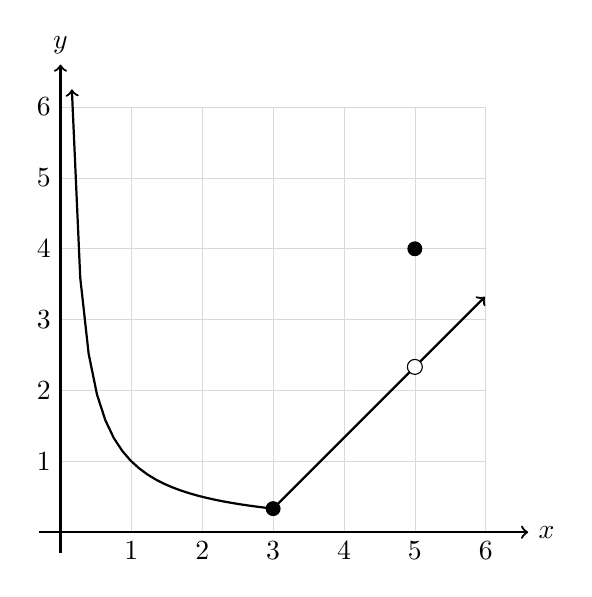
\begin{tikzpicture}[scale=0.9]
    % Grid
    \draw[step=1cm, gray!30, very thin] (0,0) grid (6,6);

    % Axes
    \draw[->, thick] (-0.3,0) -- (6.6,0) node[right]{$x$};
    \draw[->, thick] (0,-0.3) -- (0,6.6) node[above]{$y$};

    % Piecewise function with arrows
    \draw[thick, <-, domain=0.16:3] plot (\x, {1/\x});
    \draw[thick, ->, domain=3.01:5.99] plot (\x, {(\x-3)+0.333});

    % Points
    \fill (3,0.333) circle (3pt);
    \draw[fill=white] (5,2.333) circle (3pt);
    \fill (5,4) circle (3pt);

    % Tick labels
    \foreach \x in {1,2,3,4,5,6} \node[below] at (\x,0) {\x};
    \foreach \y in {1,2,3,4,5,6} \node[left] at (0,\y) {\y};
\end{tikzpicture}
\end{minipage}
\hspace{1em} % <-- controlled spacing instead of \hfill
\begin{minipage}[t]{0.40\textwidth}
\vspace{0pt}
\begin{tabular}{|c|c|c|}
    \hline
    \textbf{$x$-value} & \textbf{condition(s) violated} & \textbf{type} \\
    \hline
     & & \\
     & & \\
     & & \\
     & & \\
     & & \\
     & & \\
     & & \\
     \hline
\end{tabular}
\end{minipage}
\vspace{.25in}
\item[(b)]
\noindent
\begin{minipage}[t]{0.4\textwidth}
\vspace{0pt}
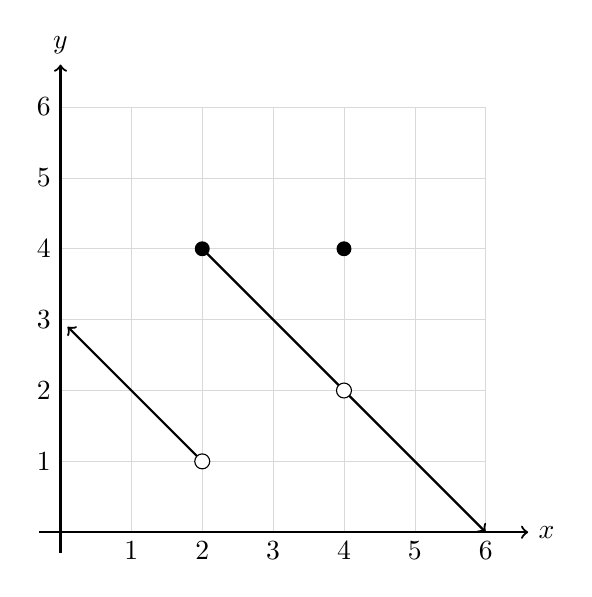
\begin{tikzpicture}[scale=0.9]
    % Grid
    \draw[step=1cm, gray!30, very thin] (0,0) grid (6,6);

    % Axes
    \draw[->, thick] (-0.3,0) -- (6.6,0) node[right]{$x$};
    \draw[->, thick] (0,-0.3) -- (0,6.6) node[above]{$y$};

    % Piecewise function with arrows
    \draw[thick, <-, domain=0.1:1.99] plot (\x, 3-\x);
    \draw[thick, ->, domain=2:6] plot (\x, -\x+2+4);

    % Points
    \draw[fill=white] (2,1) circle (3pt);
    \fill (2,4) circle (3pt);
    \draw[fill=white] (4,2) circle (3pt);
    \fill (4,4) circle (3pt);

    % Tick labels
    \foreach \x in {1,2,3,4,5,6} \node[below] at (\x,0) {\x};
    \foreach \y in {1,2,3,4,5,6} \node[left] at (0,\y) {\y};
\end{tikzpicture}
\end{minipage}
\hspace{1em} % <-- controlled spacing instead of \hfill
\begin{minipage}[t]{0.40\textwidth}
\vspace{0pt}
\begin{tabular}{|c|c|c|}
    \hline
    \textbf{$x$-value} & \textbf{condition(s) violated} & \textbf{type} \\
    \hline
     & & \\
     & & \\
     & & \\
     & & \\
     & & \\
     & & \\
     & & \\
     \hline
\end{tabular}
\end{minipage}

\vspace{.25in}
\item[(c)]
\noindent
\begin{minipage}[t]{0.4\textwidth}
\vspace{0pt}
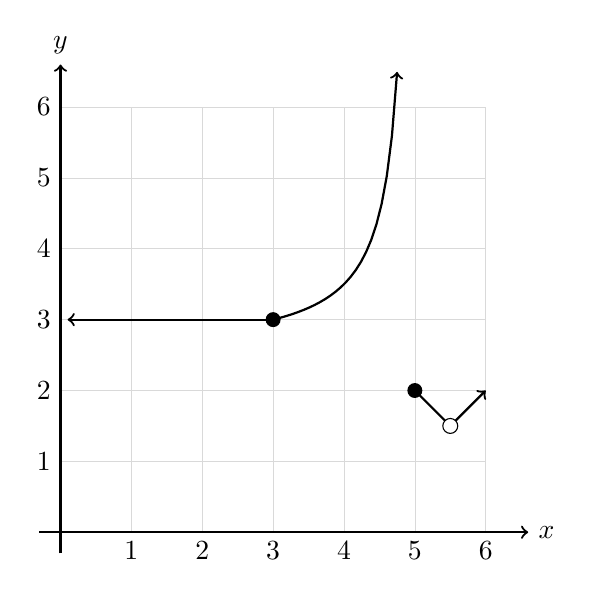
\begin{tikzpicture}[scale=0.9]
    % Grid
    \draw[step=1cm, gray!30, very thin] (0,0) grid (6,6);

    % Axes
    \draw[->, thick] (-0.3,0) -- (6.6,0) node[right]{$x$};
    \draw[->, thick] (0,-0.3) -- (0,6.6) node[above]{$y$};

    % Piecewise function with arrows
    \draw[thick, <-, domain=0.1:2.99] plot (\x, 3);
    \draw[thick, ->, domain=3:4.75] plot (\x, {3-(\x-3)/(\x-5)/2});
    \draw[thick,domain=5:5.5] plot (\x,-\x+7);
    \draw[thick, ->, domain=5.5:6] plot (\x,\x-4);

    % Points
    \fill (3,3) circle (3pt);
    \fill (5,2) circle (3pt);
    \draw[fill=white] (5.5,1.5) circle (3pt);

    % Tick labels
    \foreach \x in {1,2,3,4,5,6} \node[below] at (\x,0) {\x};
    \foreach \y in {1,2,3,4,5,6} \node[left] at (0,\y) {\y};
\end{tikzpicture}
\end{minipage}
\hspace{1em} % <-- controlled spacing instead of \hfill
\begin{minipage}[t]{0.40\textwidth}
\vspace{0pt}
\begin{tabular}{|c|c|c|}
    \hline
    \textbf{$x$-value} & \textbf{condition(s) violated} & \textbf{type} \\
    \hline
     & & \\
     & & \\
     & & \\
     & & \\
     & & \\
     & & \\
     & & \\
     \hline
\end{tabular}
\end{minipage}
\end{enumerate}
\newpage
\item[\textbf{D1.}]
A device measuring ocean temperature is placed into the ocean at time $t=0$ minutes and begins recording the temperature $T$ (in ${}^{\circ}$ C) of the ocean water as it descends.

\begin{enumerate}
    \item In terms of the context above, what does $T'(20)$ represent? What are its units of measurement? You may simply write your answers with no justification.
        \vfill
    \item In terms of the context above, what does $\displaystyle\frac{T(30)-T(20)}{30-20}$ represent? What are its units of measurement? You may simply write your answers with no justification.
        \vfill
    \item  The graph below depicts the temperature measurements of the device at different times.

    %temperature at the surface is 20 degrees C
    %held for 5 minutes then sinks at a rate of 100 meters per minute
    %after 5 minutes, its depth is still 0 and temperature is still 20
    %after 6 minutes, its depth is 100 meters
    %after 15 minutes, its depth is 1000 meters and temperature is 22-10*1=4
    %after 65 minutes, its depth is 5000 meters and temperature is 10-0.1*50=5
    
    \begin{center}
        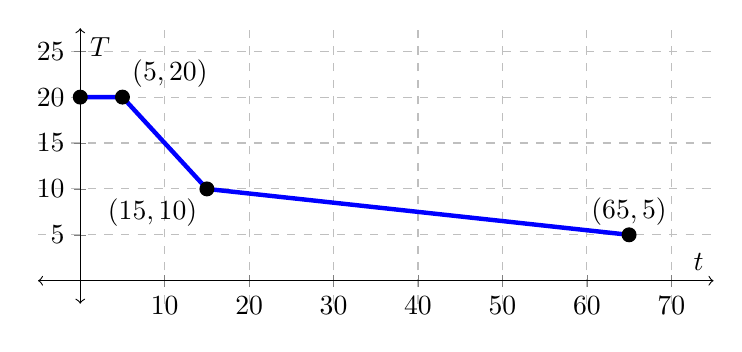
\begin{tikzpicture}
              \begin{axis}[
            %    axis y line = left,
            %    axis x line = bottom,
                xlabel = {$t$},
                ylabel = {$T$},
                ytick       = {5,10,15,20,25},
                yticklabels = {$5$,$10$,$15$,$20$,$25$},
                xtick       = {10,20,30,40,50,60,70},
                xticklabels = {$10$,$20$,$30$,$40$,$50$,$60$,$70$},
                samples     = 320,
                %domain      = 0:4,
                %restrict y to domain=-5:5,
                ymin = -2.5, ymax = 27.5,
                xmin = -5, xmax = 75,
                width=4in,height=2in,
                grid=both, grid style=dashed
              ]
             %
             \draw[ultra thick,blue] (0,20) -- (5,20) -- (15,10) -- (65,5);
             \filldraw (0,20) circle (2.5pt);
             \filldraw (5,20) circle (2.5pt) node[anchor=south west]{$(5,20)$};
             \filldraw (15,10) circle (2.5pt) node[anchor=north east]{$(15,10)$};
             \filldraw (65,5) circle (2.5pt) node[anchor=south]{$(65,5)$};
             %\addplot[blue, ultra thick, mark=none, smooth] {4-x^2};
             %
             %\addplot[blue, ultra thick, mark=none, smooth] coordinates{ (0,.61) (0.25,2.92) (0.5,0.8) (0.75,1) (1,.77) (1.25,1.34) (1.5,.74) (1.75,1.25) (2,1.47) (2.25,2.46) (2.5,3.23) (2.75,3.71) (3,5.29) (3.25,3.38) (3.5,1.11) (3.75,2.29)};
             %
             \end{axis}
        \end{tikzpicture}    
    \end{center}
    For each answer choice below, circle the answer choice if and only if the statement for that answer choice is TRUE.\\
    
    \begin{minipage}[t][1.5in]{0.2\textwidth}
        \begin{itemize}
        \item[A.] $\dfrac{dT}{dt}\bigg|_{t=3}=0$
            \vfill
        
        \item[B.] $\dfrac{dT}{dt}\bigg|_{t=3}<0$
            \vfill

        \item[C.] $\dfrac{dT}{dt}\bigg|_{t=3}>0$
            \vfill
        
        \end{itemize}
    \end{minipage}
    \hfill
    \begin{minipage}[t][1.5in]{0.2\textwidth}
        \begin{itemize}
        \item[D.] $T'(10)<0$
            \vfill

        \item[E.] $T'(10)>0$
            \vfill

        \item[F.] $T'(10)=0$
            \vfill
        
        \end{itemize}
    \end{minipage}        
        
\end{enumerate}
\newpage
\begin{itemize}
\item\textbf{First Derivative Test.}
Suppose that $c$ is a
\textbf{critical number}
of a continuous function $f$.
\begin{enumerate}
\item
If $f'$ changes from
\textbf{positive}
to
\textbf{negative}
at $c$, then $f$ has a
\textbf{local maximum} at $c$.
\item
If $f'$ changes from
\textbf{negative}
to
\textbf{positive}
at $c$, then $f$ has a
\textbf{local minimum}
at $c$.
\item
If $f'$ does not change sign at $c$,
then $f$ has
\textbf{neither local maximum, nor local minimum}
at $c$.
\end{enumerate}
\vfill
\item\textbf{Second Derivative Test.}
Suppose $f''$ is continuous near a critical number $x=c$.
\begin{enumerate}
\item
If \textbf{$f^{\prime}(c)=0$ and $f^{\prime\prime}(c)<0$}
then we have a
\textbf{local maximum at $x=c$}.
\item
If \textbf{$f^{\prime}(c)=0$ and $f^{\prime\prime}(c)>0$}
then we have a
\textbf{local minimum at $x=c$}.
\item
If \textbf{$f^{\prime}(c)$ DNE,
$f^{\prime\prime}(c)=0$, or
$f^{\prime\prime}(c)$ DNE}
then we cannot use the Second Derivative Test\\
(i.e. the \textbf{test is inconclusive}).
\end{enumerate}
\vfill
\item
\textbf{Closed Interval Method.}
To find the absolute maximum value and absolute minimum value of a continuous function $f$ on the closed interval $[a, b]$, do the following:
\smallskip

\begin{minipage}{0.75\textwidth}
\begin{enumerate}
\item  Find the critical numbers $c_1, c_2, \ldots, c_n$ of $f$ that lie in $(a, b)$.
\item  Find the value of $f$ at each critical number {\em and} at the endpoints


\item  The largest value from (b)  will be the absolute maximum value of $f$ on $[a, b]$ and the smallest value from (b) will be the absolute minimum value of $f$ on $[a, b]$. 
\end{enumerate}
\end{minipage}
%
\hfill
%
\begin{minipage}{0.2\textwidth}
\begin{center}
\begin{tabular}{|c|c|}
\hline 
$x$ & $f(x)$\tabularnewline
\hline 
\hline 
$a$ & $f(a)$\tabularnewline
\hline 
$b$ & $f(b)$\tabularnewline
\hline 
$c_1$ & $f(c_1)$\tabularnewline
\hline 
$c_2$ & $f(c_2)$\tabularnewline
\hline 
$\vdots$ &$\vdots $\tabularnewline
\hline 
$c_n$ & $f(c_n)$\tabularnewline
\hline 
\end{tabular}
\end{center}
\end{minipage}
\vfill
\item
\textbf{First Derivative Test for Absolute Extrema.}
Suppose that $c$ is a critical number of a continuous function $f$ defined on an interval $I$.
    \begin{itemize}
    \item {\bf If} the sign of $f'$ changes from positive ($+$) to negative ($-$) at $c$ {\bf and} $c$ is the only critical number where $f^{\prime}$ changes sign on $I$
    %\emph{and} if $c$ is the only $x$-value in $I$ at which $f$ changes sign, 
    {\bf then} $f(c)$ is the absolute maximum value of $f$ on $I$.
    \item {\bf If} the sign of $f'$ changes from negative ($-$) to positive ($+$) at $c$ {\bf and} $c$ is the only critical number where $f^{\prime}$ changes sign on $I$
    % \emph{and} if $c$ is the only $x$-value in $I$ at which $f$ changes sign, 
    {\bf then} $f(c)$ is the absolute minimum value of $f$ on $I$.\\
    \end{itemize}
\end{itemize}
\newpage
\item[\textbf{A1.}]
This problem pertains to the following graph:

\begin{center}
    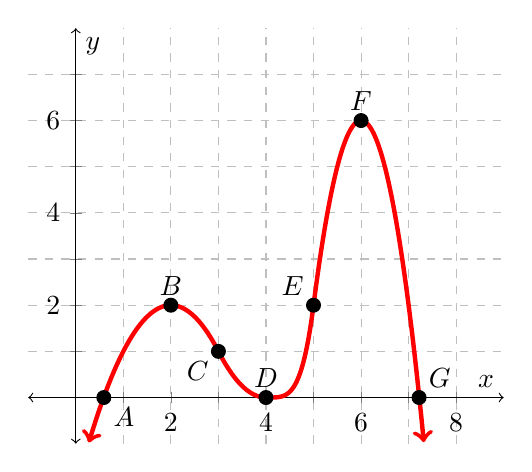
\begin{tikzpicture}[scale=1]
          \begin{axis}[
            xlabel={$x$},
            %grid = major,
            xtick       = {1,2,3,4,5,6,7,8},
            xticklabels = { ,$2$, ,$4$, ,$6$, ,$8$},
            ytick       = {1,2,3,4,5,6,7},
            yticklabels = { ,$2$, ,$4$, ,$6$, },
            samples     = 320,
            domain      = -1:9,
            restrict y to domain=-1:8,
            xmin = -1, xmax = 9,
            ymin = -1, ymax = 8,
            height=2.7in, width=3in,
            grid=both,grid style=dashed
          ]
          % old version of the curve
          %
          %\addplot[domain=-1:9, purple, ultra thick, mark=none] {-1/10*(x-1)*(x-4)^2*(x-7)};
          %
          %new version of the curve in pieces
          %
          \addplot[domain=0.25:3, ultra thick, red, <-] {2-(x-2)^2};
          \addplot[domain=3:4, ultra thick, red] {(x-4)^2};
          \addplot[domain=4:5, ultra thick, red] {2*(x-4)^4};
          %\addplot[domain=5:6, ultra thick, red] {4*(x-5)};
          \addplot[domain=5:9, ultra thick, red,->] {-4*(x-6)^2+6};
          \filldraw (.59,0) circle (2.5pt) node[anchor=north west]{$A$};
          \filldraw (2,2) circle (2.5pt) node[anchor=south]{$B$};
          \filldraw (3,1) circle (2.5pt) node[anchor=north east]{$C$};
          \filldraw (4,0) circle (2.5pt) node[anchor=south]{$D$};
          \filldraw (5,2) circle (2.5pt) node[anchor=south east]{$E$};
          \filldraw (6,6) circle (2.5pt) node[anchor=south]{$F$};
          \filldraw (7.22,0) circle (2.5pt) node[anchor=south west]{$G$};
          %
        \end{axis}
    \end{tikzpicture}
\end{center}

Use the 7 labeled points together with ``H. None of the other answers" as answer choices for the following questions. You may simply write your answers.

    \begin{enumerate}
        \item At which points would both $\dfrac{df}{dx}$ and $\dfrac{d^2f}{dx^2}$ be positive if the given graph were the graph of the function $f$? Provide all correct answers.\\

        \begin{center}
        {\large Answer(s):} \rule[-8pt]{3in}{0.4pt}
        \end{center}

        \vfill

        \item At which points would both $\dfrac{df}{dx}$ and $\dfrac{d^2f}{dx^2}$ be positive if the given graph were the graph of the derivative $f'$? Provide all correct answers.\\

        \begin{center}
        {\large Answer(s):} \rule[-8pt]{3in}{0.4pt}
        \end{center}

        \vfill
        
        \item At which points would $f$ have a critical number if the given graph were the graph of the derivative $f'$?\\

        \begin{center}
        {\large Answer(s):} \rule[-8pt]{3in}{0.4pt}
        \end{center}

        \vfill
        
        \item At which points would $f$ have an inflection point if the given graph were the graph of the second derivative $f''$?\\

        \begin{center}
        {\large Answer(s):} \rule[-8pt]{3in}{0.4pt}
        \end{center}

        \vfill
        
    \end{enumerate}
\newpage
\item[\textbf{A2.}]
\[f(x)=2x^{3/2}-x\]

\begin{enumerate}
\item Finde the domain of $f(x)$.
\item Find all critical numbers of $f(x)$.
\vfill
\item Find the $x$-values of all absolute extrema of $f(x)$ on the interval $[-1, 8]$.
\vfill
\end{enumerate}
\newpage
\item[\textbf{A3.}]
We have a piece of cardboard that is $14$ inches by $10$ inches and we are going to cut out the corners as shown below and fold up the sides to form a box, also shown below. Determine the height of the box that will give a maximum volume.
\begin{center}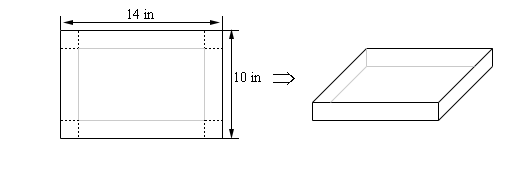
\includegraphics[width=0.75\textwidth]{../../images/cardboard_box_height.png}\end{center}
\newpage
\item[\textbf{I1.}]
You may simply record your answers with no work shown. Please show your work to part (b). ({\bf Note:} Below, ``NOTOA" means ``none of the other answers".)
        \begin{itemize}

    \item[(a)] Suppose $f$ is a continuous function of the variable $t$, $0\leq t\leq 24$. If $f$ is measured in megawatts (MW) and $t$ is measured in hours (hr), then what are the units of $\displaystyle\int_0^{24} f(t)\,dt$?\\

    \,\hfill
    \fbox{A} MW/hr$^2$
    \hfill
    \fbox{B} MW/hr
    \hfill
    \fbox{C} MW
    \hfill
    \fbox{D} hr
    \hfill
    \fbox{E} NOTOA
    \hfill\,\\
\medskip{}

    \item[(b)] If $p(t)$ represents the (instantaneous) rate of change of levels (in parts per million) of an airborne pollutant $t$ hours after midnight on a given day, then what does $\displaystyle\int_6^{12} p(t)\,dt$ represent in this context?
        \vspace{6cm}

    \item[(c)] Let $T'(t)$ represent the (instantaneous) rate of change (in $^{\circ}$C/hour) of temperature in Charlottesville at a time $t$ (in hours) during a particular day. Assume the temperature was highest at 5:00 PM and lowest at 4:00 AM. Which of the following integrals are {\bf positive}? Circle all correct answers.\\[0.2in]
    %
    \,\hfill
    \fbox{A} $\displaystyle\int_{12}^{17} T'(x)\,dx$
    \hfill
    \fbox{B} $\displaystyle\int_{17}^{22} T'(x)\,dx$
    \hfill
    \fbox{C} $\displaystyle\int_1^4 T'(x)\,dx$
    \hfill
    \fbox{D} $\displaystyle\int_4^{10} T'(x)\,dx$
    \hfill
    \fbox{E} NOTOA        
\end{itemize}

%%%%%%%%%%%%%%%%%%%%%%%%%%%%%%%%%%%%%%%%%%%%%%%%%%%%%
%%%%%%%%%%% END PROBLEM I1 %%%%%%%%%%%%%%%%%%%%%%%%%%
%%%%%%%%%%%%%%%%%%%%%%%%%%%%%%%%%%%%%%%%%%%%%%%%%%%%%
\newpage
%%%%%%%%%%%%%%%%%%%%%%%%%%%%%%%%%%%%%%%%%%%%%%%%%%%%%
%%%%%%%%%%% BEGIN PROBLEM I2 %%%%%%%%%%%%%%%%%%%%%%%%
%%%%%%%%%%%%%%%%%%%%%%%%%%%%%%%%%%%%%%%%%%%%%%%%%%%%%

\item[\textbf{I2.}]

The graph of $f(x)$ is given below.

\begin{center}
    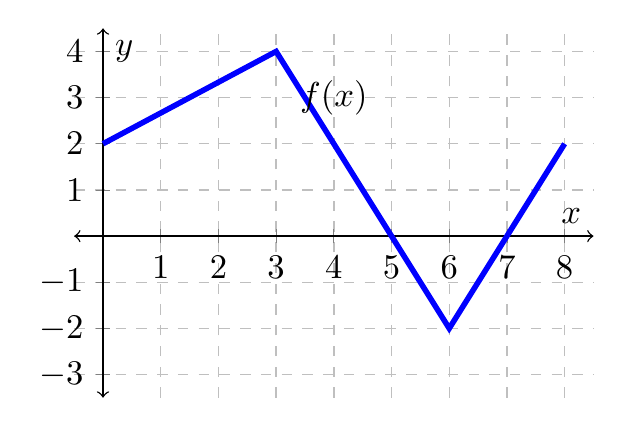
\begin{tikzpicture}[scale=1.25]
          \begin{axis}[
            xlabel={$x$},
            %grid = major,
            xtick       = {1,2,3,4,5,6,7,8},
            xticklabels = {$1$,$2$,$3$,$4$,$5$,$6$,$7$,$8$},
            ytick       = {-3, -2, -1, 0,1,2,3,4},
            yticklabels = {$-3$, $-2$, $-1$, $0$,$1$,$2$,$3$,$4$},
            samples     = 320,
            domain      = -1:9.5,
            restrict y to domain=-3.5:2.5,
            xmin = -0.5, xmax = 8.5,
            ymin = -3.5, ymax = 4.5,
            height=2.1in, width=2.7in,
            grid=both, grid style=dashed
          ]
          \draw[ultra thick, blue] (0,2) -- (3,4) -- (6,-2) -- (8, 2);
          \node at (4,3) {$f(x)$};
          \end{axis}
    \end{tikzpicture}
    \end{center}

    In addition, we know that $g(x)$ satisfies the following.

    \[\int_5^3g(x)=-2\,dx\]

    \[\int_0^3g(x)=10\,dx\]

    Find the values of the following integrals.

    \begin{enumerate}
        \item $\displaystyle\int_5^7f(x)\,dx$

        \vfill

        \item $\displaystyle\int_3^52f(x)-g(x)\,dx$

        \vfill

        \item $\displaystyle\int_0^5 2f(x)-g(x)\,dx$

        \vfill
    \end{enumerate}

%%%%%%%%%%%%%%%%%%%%%%%%%%%%%%%%%%%%%%%%%%%%%%%%%%%%%
%%%%%%%%%%% END PROBLEM I2 %%%%%%%%%%%%%%%%%%%%%%%%%%
%%%%%%%%%%%%%%%%%%%%%%%%%%%%%%%%%%%%%%%%%%%%%%%%%%%%%

\newpage

%%%%%%%%%%%%%%%%%%%%%%%%%%%%%%%%%%%%%%%%%%%%%%%%%%%%%
%%%%%%%%%%% BEGIN PROBLEM I3 %%%%%%%%%%%%%%%%%%%%%%%%
%%%%%%%%%%%%%%%%%%%%%%%%%%%%%%%%%%%%%%%%%%%%%%%%%%%%%

\item[\textbf{I3.}]
Assume $x>0$. Write down the indefinite integrals of the following expressions. 

Although no work is required, you are encouraged to include any work that shows your thought process. 

%constant, power, exponential, log, +C, algebraic manipulation

\begin{center}
        \begin{tabular}{l c r l c r}
            %
            $\displaystyle\int 9x^{10}\,dx$ & $=$ & \rule[-8pt]{1.5in}{0.4pt} &
            %
            $\displaystyle\int \dfrac{1}{x^2} \,dx$ & $=$ & \rule[-8pt]{1.5in}{0.4pt}\\[1in]
            %%%%%
            $\displaystyle\int \dfrac{3}{x}-2\,dx$ & $=$ & \rule[-8pt]{1.5in}{0.4pt}&
            %
            $\displaystyle\int 2^x\,dx$ & $=$ & \rule[-8pt]{1.5in}{0.4pt}\\[1in]
            %%%%%
            $\displaystyle\int e^x+\sqrt[3]{x} \,dx$ & $=$ & \rule[-8pt]{1.5in}{0.4pt} & 
            %
            $\displaystyle\int \dfrac{1}{\sqrt{x^5}} \,dx$ & $=$ & \rule[-8pt]{1.5in}{0.4pt}\\[0.3in]
            %%%%%
        \end{tabular}
\end{center}

%%%%%%%%%%%%%%%%%%%%%%%%%%%%%%%%%%%%%%%%%%%%%%%%%%%%%
%%%%%%%%%%% END PROBLEM I3 %%%%%%%%%%%%%%%%%%%%%%%%%%
%%%%%%%%%%%%%%%%%%%%%%%%%%%%%%%%%%%%%%%%%%%%%%%%%%%%%

\newpage

%%%%%%%%%%%%%%%%%%%%%%%%%%%%%%%%%%%%%%%%%%%%%%%%%%%%%
%%%%%%%%%%% BEGIN PROBLEM I4 %%%%%%%%%%%%%%%%%%%%%%%%
%%%%%%%%%%%%%%%%%%%%%%%%%%%%%%%%%%%%%%%%%%%%%%%%%%%%%

\item[\textbf{I4.}]
\begin{enumerate}

            \item On which of the following integrals could the Fundamental Theorem of Calculus NOT be used? Circle \textbf{all} the correct answers, and then evaluate the remaining ones.

    \,\hfill
    \fbox{A} $\displaystyle\int_{-1}^1 \ln (x^2)\,dx$
    \hfill
    \fbox{B} $\displaystyle\int_{-1}^3 \frac1{x^2-4}\,dx$
    \hfill
    \fbox{C} $\displaystyle\int_{2}^{-4} 2^x\,dx$
    \hfill
    \fbox{D} $\displaystyle\int_{-2}^{0} e^{\sqrt{x}}\,dx$
    \hfill\

    \vspace{5cm}

\item Evaluate the integral:
    \[
        \int_{1}^3 \frac{x+2x^2}{x^2}\,dx
    \]
        \end{enumerate}
        \pagebreak

%%%%%%%%%%%%%%%%%%%%%%%%%%%%%%%%%%%%%%%%%%%%%%%%%%%%%
%%%%%%%%%%% END PROBLEM I4 %%%%%%%%%%%%%%%%%%%%%%%%%%
%%%%%%%%%%%%%%%%%%%%%%%%%%%%%%%%%%%%%%%%%%%%%%%%%%%%%
\end{enumerate}

\end{document}